\begin{figure}[t]
\centering
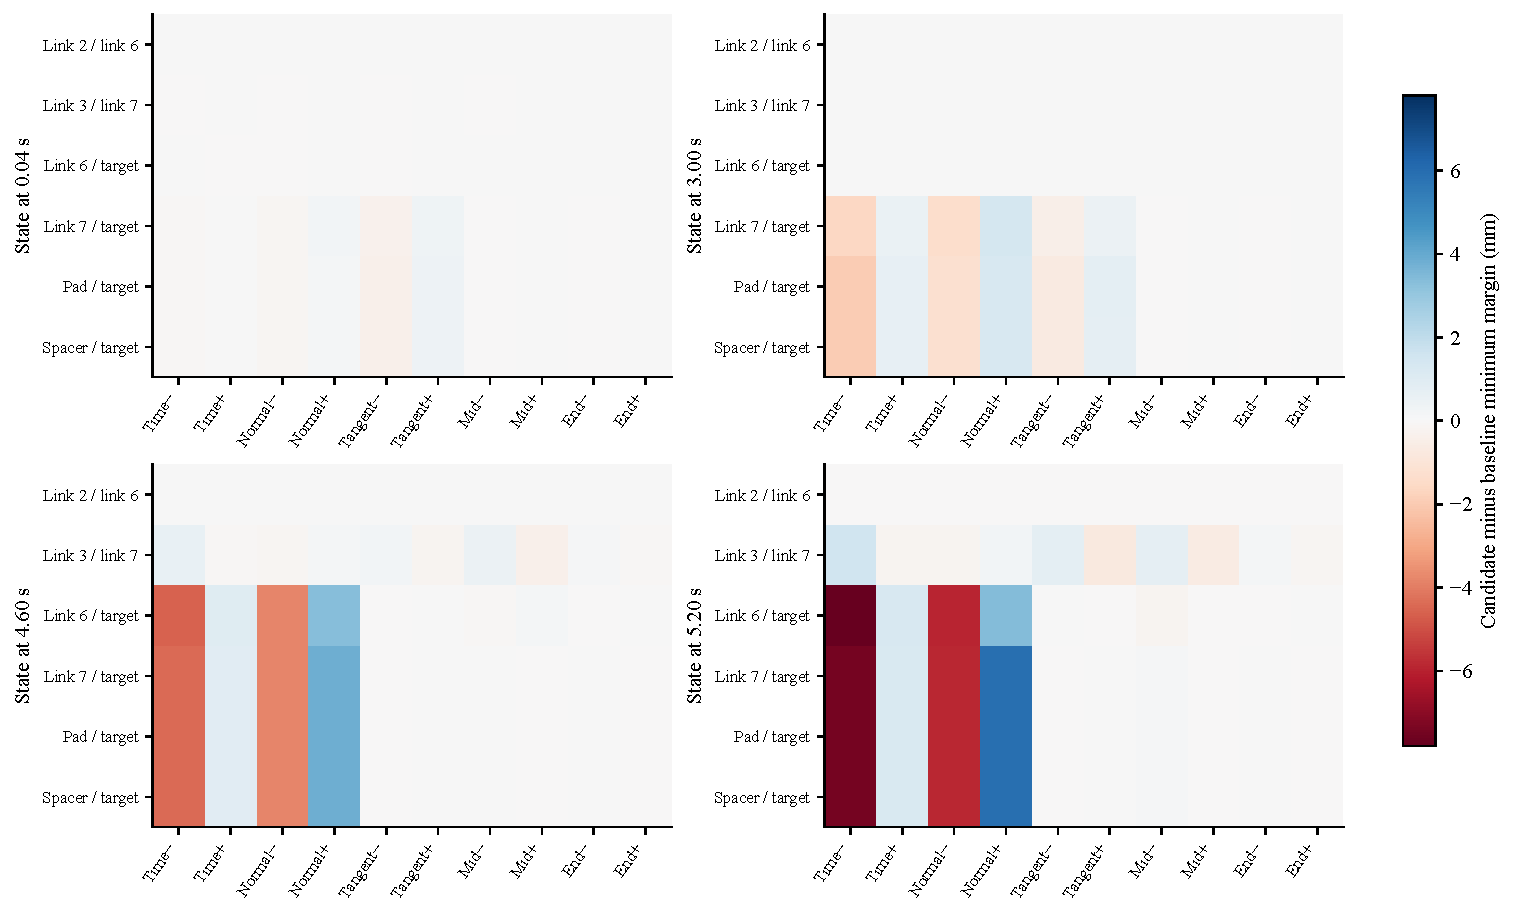
\includegraphics[width=0.95\linewidth]{authority_signed.pdf}
\caption{Signed changes for six named pairs at four preregistered B01 states, each using the same 0.6 s prior forecast. Columns change one dimension with its negative/positive perturbation. Positive means increased predicted minimum distance, not task success. All finite pairs and thresholds are in authority\_signed\_margins.csv; absent-distance sentinels are excluded.}
\label{fig:s03-authority-signed}
\end{figure}

\begin{figure}[t]
\centering
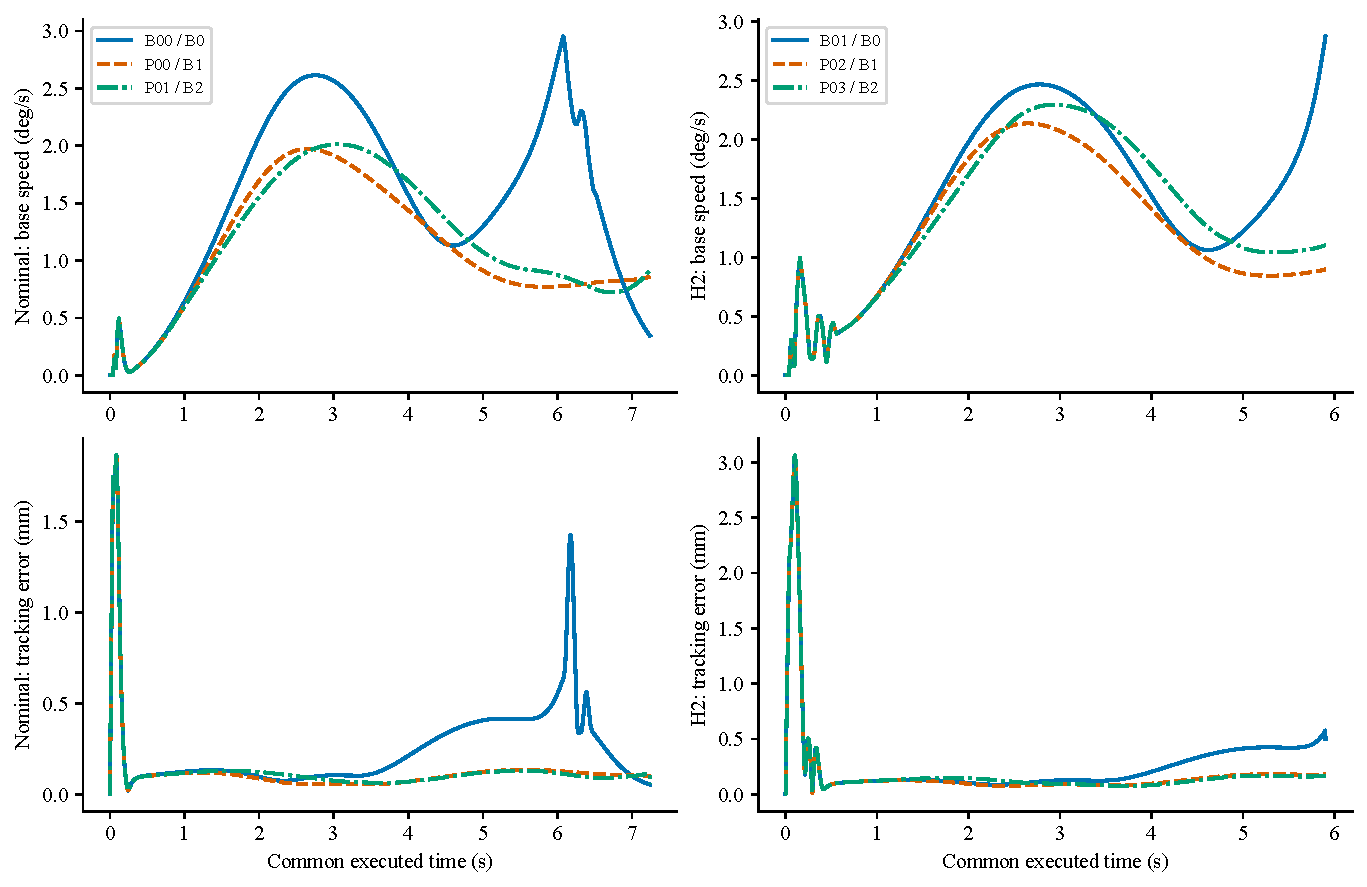
\includegraphics[width=0.95\linewidth]{common_prefix.pdf}
\caption{B0/B1/B2 actual base angular speed and active-reference tracking error, truncated to the shortest executed interval in each scene. This figure excludes later baseline capture and does not establish complete-task benefit, risk reduction or postgrasp performance. Runs are deterministic seen-condition comparisons, not independent statistical samples.}
\label{fig:s03-common-prefix}
\end{figure}

\begin{figure}[t]
\centering
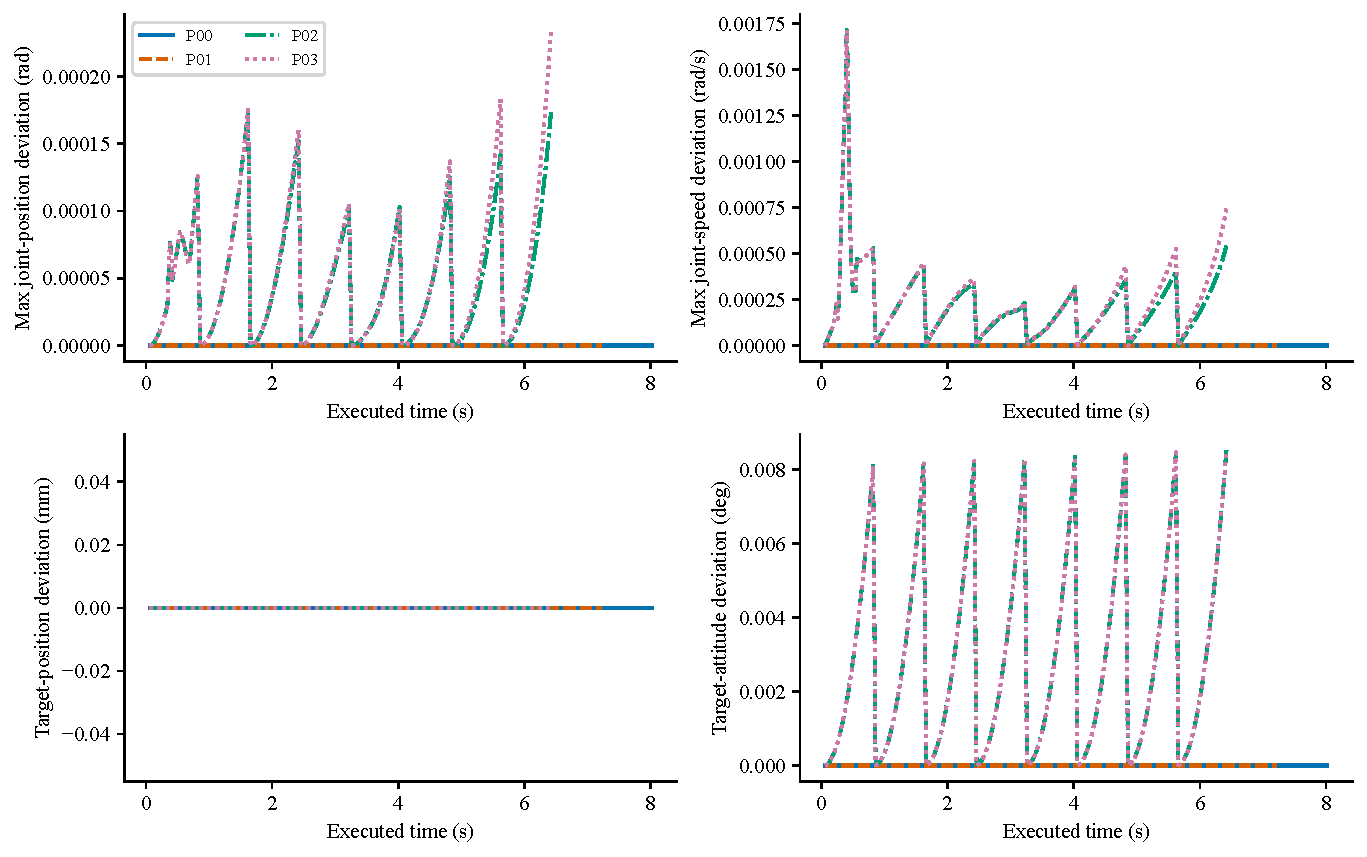
\includegraphics[width=0.95\linewidth]{forecast_errors.pdf}
\caption{Public joint measurements and CA18 target estimates against the selected independent-prior cached forecast at actual cache-validation ticks. Traces end at the last cache check before termination (P00/P01/P02/P03: 8.02/7.22/6.42/6.42 s). Replanning resets the forecast horizon. These are cache-domain diagnostics, not a global prediction error guarantee; truth is not fed to the planner.}
\label{fig:s03-forecast-errors}
\end{figure}
